% ============================================================
% CHAPTER 2: Sprint 1 & Sprint 2 — Landing Page + Authentication
% ============================================================
% ADD THIS TO main.tex AFTER COMPLETING SPRINT 1 & 2
% Uncomment: % ============================================================
% CHAPTER 2: Sprint 1 & Sprint 2 — Landing Page + Authentication
% ============================================================
% ADD THIS TO main.tex AFTER COMPLETING SPRINT 1 & 2
% Uncomment: % ============================================================
% CHAPTER 2: Sprint 1 & Sprint 2 — Landing Page + Authentication
% ============================================================
% ADD THIS TO main.tex AFTER COMPLETING SPRINT 1 & 2
% Uncomment: % ============================================================
% CHAPTER 2: Sprint 1 & Sprint 2 — Landing Page + Authentication
% ============================================================
% ADD THIS TO main.tex AFTER COMPLETING SPRINT 1 & 2
% Uncomment: \input{chapters/chapter2}
% ============================================================
\chapter{Sprint 1 \& Sprint 2: Foundation and Authentication}

\section{Introduction}

This chapter covers the first two sprints of the project. Sprint 1 focuses on establishing the project foundation and building the landing page, while Sprint 2 implements the authentication service with JWT-based security.

% ============================================================
% SPRINT 1
% ============================================================
\section{Sprint 1: Landing Page \& Project Foundation}

\sprintcard{1}{Landing Page \& Project Foundation}{Deliver a responsive landing page and set up the project skeleton with Docker containers.}

\subsection{Sprint Backlog}

\begin{longtable}{|c|p{5cm}|c|c|c|}
\hline
\rowcolor{blue!15}
\textbf{Task ID} & \textbf{Task} & \textbf{Assignee} & \textbf{Est.} & \textbf{Status} \\
\hline
\endhead
T-1.1 & Scaffold Next.js project & DSI & 2h & Done \\
\hline
T-1.2 & Scaffold NestJS microservices & DSI & 4h & Done \\
\hline
T-1.3 & Setup Docker Compose & DSI & 3h & Done \\
\hline
T-1.4 & Setup PostgreSQL + ORM & DSI & 3h & Done \\
\hline
T-1.5 & Landing page — Hero section & DSI & 4h & Done \\
\hline
T-1.6 & Landing page — Pricing section & DSI & 4h & Done \\
\hline
T-1.7 & Landing page — Features + Footer & DSI & 3h & Done \\
\hline
T-1.8 & Responsive design + Polish & DSI & 4h & Done \\
\hline
T-1.9 & Ubuntu Server hardening & RSI & 4h & Done \\
\hline
T-1.10 & Network configuration & RSI & 3h & Done \\
\hline
T-1.11 & Docker install on server & RSI & 2h & Done \\
\hline
T-1.12 & OpenNebula research & RSI & 6h & Done \\
\hline
\caption{Sprint 1 backlog}
\label{tab:sprint1-backlog}
\end{longtable}

\subsection{Mockups and Design}

% INSERT FIGMA SCREENSHOTS HERE
\begin{figure}[H]
\centering
% \includegraphics[width=\textwidth]{images/landing-mockup.png}
\fbox{\parbox{0.9\textwidth}{\centering\vspace{3cm}\textit{Insert Figma landing page mockup here}\vspace{3cm}}}
\caption{Landing page mockup (Figma)}
\label{fig:landing-mockup}
\end{figure}

\subsection{Implementation}

\subsubsection{Project Structure}

The project follows a monorepo structure with separate directories for each microservice:

\begin{lstlisting}[language=bash, caption={Project directory structure}]
cloudvm/
├── frontend/          # Next.js application
├── services/
│   ├── gateway/       # API Gateway (NestJS)
│   ├── auth/          # Auth Service (NestJS)
│   ├── user/          # User Service (NestJS)
│   ├── vm/            # VM Service (NestJS)
│   └── payment/       # Payment Service (NestJS)
├── worker/            # Python Worker
├── docker-compose.yml
└── .env
\end{lstlisting}

\subsubsection{Landing Page Screenshots}

% INSERT ACTUAL SCREENSHOTS HERE
\begin{figure}[H]
\centering
\fbox{\parbox{0.9\textwidth}{\centering\vspace{3cm}\textit{Insert landing page hero section screenshot}\vspace{3cm}}}
\caption{Landing page — Hero section}
\label{fig:landing-hero}
\end{figure}

\begin{figure}[H]
\centering
\fbox{\parbox{0.9\textwidth}{\centering\vspace{3cm}\textit{Insert landing page pricing section screenshot}\vspace{3cm}}}
\caption{Landing page — Pricing section}
\label{fig:landing-pricing}
\end{figure}

\subsection{Sprint 1 Review}

At the end of Sprint 1, the following deliverables were achieved:
\begin{itemize}
  \item Responsive landing page with hero, features, pricing, and footer sections.
  \item Docker Compose configuration with containers for all microservices.
  \item PostgreSQL database initialized with ORM configuration.
  \item Ubuntu Server hardened with SSH key authentication.
  \item Docker installed and configured on the server.
\end{itemize}


% ============================================================
% SPRINT 2
% ============================================================
\section{Sprint 2: Authentication Service}

\sprintcard{2}{Authentication Service}{Implement secure user registration, login, JWT authentication, and role-based access control.}

\subsection{Sprint Backlog}

\begin{longtable}{|c|p{5cm}|c|c|c|}
\hline
\rowcolor{blue!15}
\textbf{Task ID} & \textbf{Task} & \textbf{Assignee} & \textbf{Est.} & \textbf{Status} \\
\hline
\endhead
T-2.1 & Registration endpoint & DSI & 4h & Done \\
\hline
T-2.2 & Login endpoint & DSI & 4h & Done \\
\hline
T-2.3 & JWT + Refresh tokens & DSI & 4h & Done \\
\hline
T-2.4 & Logout + token blacklist & DSI & 2h & Done \\
\hline
T-2.5 & Password reset flow & DSI & 3h & Done \\
\hline
T-2.6 & Auth guards (JWT, Role) & DSI & 3h & Done \\
\hline
T-2.7 & Register page (frontend) & DSI & 4h & Done \\
\hline
T-2.8 & Login page (frontend) & DSI & 3h & Done \\
\hline
T-2.9 & Auth state management & DSI & 3h & Done \\
\hline
T-2.10 & OpenNebula installation & RSI & 6h & Done \\
\hline
T-2.11 & OpenNebula configuration & RSI & 6h & Done \\
\hline
T-2.12 & KVM setup + VM templates & RSI & 6h & Done \\
\hline
\caption{Sprint 2 backlog}
\label{tab:sprint2-backlog}
\end{longtable}

\subsection{Use Case Diagram — Authentication}

\begin{figure}[H]
\centering
\begin{tikzpicture}[
  usecase/.style={draw, ellipse, minimum width=3cm, minimum height=0.8cm, align=center, font=\scriptsize}
]
  % System boundary
  \draw[thick, rounded corners] (0, -5) rectangle (6, 0.5);
  \node[font=\small\bfseries] at (3, 0.2) {Authentication Module};
  
  % Actor
  \node (visitor) at (-2, -2) {Visitor};
  
  % Use cases
  \node[usecase] (uc1) at (3, -0.5) {Register};
  \node[usecase] (uc2) at (3, -1.5) {Login};
  \node[usecase] (uc3) at (3, -2.5) {Logout};
  \node[usecase] (uc4) at (3, -3.5) {Reset Password};
  \node[usecase] (uc5) at (3, -4.5) {Refresh Token};
  
  % Arrows
  \draw (visitor) -- (uc1);
  \draw (visitor) -- (uc2);
  \draw (visitor) -- (uc3);
  \draw (visitor) -- (uc4);
  \draw[dashed] (uc2) -- node[right, font=\tiny] {<<include>>} (uc5);
  
\end{tikzpicture}
\caption{Use case diagram — Authentication}
\label{fig:uc-auth}
\end{figure}

\subsection{Sequence Diagram — Registration}

\begin{figure}[H]
\centering
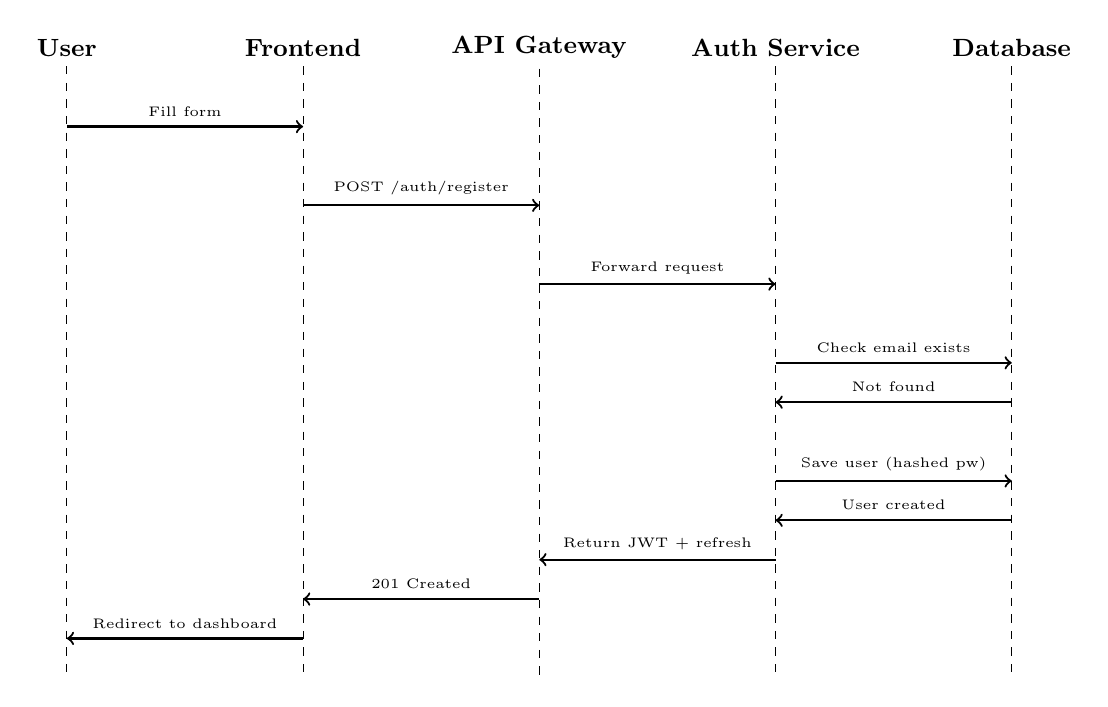
\begin{tikzpicture}[font=\small]
  % Lifelines
  \node (user) at (0, 0) {\textbf{User}};
  \node (front) at (3, 0) {\textbf{Frontend}};
  \node (gate) at (6, 0) {\textbf{API Gateway}};
  \node (auth) at (9, 0) {\textbf{Auth Service}};
  \node (db) at (12, 0) {\textbf{Database}};
  
  \draw[dashed] (user) -- (0, -8);
  \draw[dashed] (front) -- (3, -8);
  \draw[dashed] (gate) -- (6, -8);
  \draw[dashed] (auth) -- (9, -8);
  \draw[dashed] (db) -- (12, -8);
  
  % Messages
  \draw[->, thick] (0, -1) -- node[above, font=\tiny] {Fill form} (3, -1);
  \draw[->, thick] (3, -2) -- node[above, font=\tiny] {POST /auth/register} (6, -2);
  \draw[->, thick] (6, -3) -- node[above, font=\tiny] {Forward request} (9, -3);
  \draw[->, thick] (9, -4) -- node[above, font=\tiny] {Check email exists} (12, -4);
  \draw[<-, thick] (9, -4.5) -- node[above, font=\tiny] {Not found} (12, -4.5);
  \draw[->, thick] (9, -5.5) -- node[above, font=\tiny] {Save user (hashed pw)} (12, -5.5);
  \draw[<-, thick] (9, -6) -- node[above, font=\tiny] {User created} (12, -6);
  \draw[<-, thick] (6, -6.5) -- node[above, font=\tiny] {Return JWT + refresh} (9, -6.5);
  \draw[<-, thick] (3, -7) -- node[above, font=\tiny] {201 Created} (6, -7);
  \draw[<-, thick] (0, -7.5) -- node[above, font=\tiny] {Redirect to dashboard} (3, -7.5);
\end{tikzpicture}
\caption{Sequence diagram — User registration}
\label{fig:seq-register}
\end{figure}

\subsection{Sequence Diagram — Login}

\begin{figure}[H]
\centering
\begin{tikzpicture}[font=\small]
  % Lifelines
  \node (user) at (0, 0) {\textbf{User}};
  \node (front) at (3, 0) {\textbf{Frontend}};
  \node (gate) at (6, 0) {\textbf{API Gateway}};
  \node (auth) at (9, 0) {\textbf{Auth Service}};
  \node (db) at (12, 0) {\textbf{Database}};
  
  \draw[dashed] (user) -- (0, -8);
  \draw[dashed] (front) -- (3, -8);
  \draw[dashed] (gate) -- (6, -8);
  \draw[dashed] (auth) -- (9, -8);
  \draw[dashed] (db) -- (12, -8);
  
  % Messages
  \draw[->, thick] (0, -1) -- node[above, font=\tiny] {Enter credentials} (3, -1);
  \draw[->, thick] (3, -2) -- node[above, font=\tiny] {POST /auth/login} (6, -2);
  \draw[->, thick] (6, -3) -- node[above, font=\tiny] {Forward request} (9, -3);
  \draw[->, thick] (9, -4) -- node[above, font=\tiny] {Find user by email} (12, -4);
  \draw[<-, thick] (9, -4.5) -- node[above, font=\tiny] {User found} (12, -4.5);
  \draw[->, thick] (9, -5) -- node[right, font=\tiny] {Compare passwords};
  \draw[->, thick] (9, -5.5) -- node[right, font=\tiny] {Generate JWT + refresh};
  \draw[<-, thick] (6, -6) -- node[above, font=\tiny] {Return tokens} (9, -6);
  \draw[<-, thick] (3, -6.5) -- node[above, font=\tiny] {200 OK + tokens} (6, -6.5);
  \draw[<-, thick] (0, -7) -- node[above, font=\tiny] {Store token, redirect} (3, -7);
\end{tikzpicture}
\caption{Sequence diagram — User login}
\label{fig:seq-login}
\end{figure}

\subsection{Class Diagram — Auth Module}

\begin{figure}[H]
\centering
\begin{tikzpicture}[font=\small,
  class/.style={draw, rectangle, minimum width=4cm, align=left}
]
  % User class
  \node[class, fill=yellow!15] (userclass) at (0, 0) {
    \textbf{User}\\
    \hline
    - id: UUID\\
    - email: String\\
    - password: String\\
    - firstName: String\\
    - lastName: String\\
    - role: Role\\
    - createdAt: DateTime\\
    - updatedAt: DateTime\\
    \hline
    + register()\\
    + login()\\
    + resetPassword()
  };
  
  % Role enum
  \node[class, fill=green!15] (roleenum) at (6, 0) {
    \textbf{<<enum>> Role}\\
    \hline
    USER\\
    ADMIN
  };
  
  % RefreshToken class
  \node[class, fill=blue!15] (tokenclass) at (0, -5.5) {
    \textbf{RefreshToken}\\
    \hline
    - id: UUID\\
    - token: String\\
    - userId: UUID\\
    - expiresAt: DateTime\\
    - isRevoked: Boolean\\
    \hline
    + revoke()
  };
  
  % Relations
  \draw[->, thick] (userclass) -- node[above, font=\tiny] {has} (roleenum);
  \draw[->, thick] (userclass) -- node[left, font=\tiny] {has many} (tokenclass);
\end{tikzpicture}
\caption{Class diagram — Authentication module}
\label{fig:class-auth}
\end{figure}

\subsection{Implementation Screenshots}

% INSERT ACTUAL SCREENSHOTS HERE
\begin{figure}[H]
\centering
\fbox{\parbox{0.9\textwidth}{\centering\vspace{3cm}\textit{Insert registration page screenshot}\vspace{3cm}}}
\caption{Registration page}
\label{fig:register-page}
\end{figure}

\begin{figure}[H]
\centering
\fbox{\parbox{0.9\textwidth}{\centering\vspace{3cm}\textit{Insert login page screenshot}\vspace{3cm}}}
\caption{Login page}
\label{fig:login-page}
\end{figure}

\subsection{Sprint 2 Review}

At the end of Sprint 2, the following deliverables were achieved:
\begin{itemize}
  \item Complete auth service with registration, login, logout, password reset.
  \item JWT + refresh token implementation with role-based guards.
  \item Login and registration pages with form validation.
  \item OpenNebula installed and configured on the server.
  \item KVM hypervisor operational with VM templates.
\end{itemize}

% ============================================================
\section{Conclusion}

In this chapter, we completed the first two sprints. Sprint 1 established the project foundation with a modern landing page and Docker-based development environment. Sprint 2 delivered a complete authentication system with secure JWT-based access control. On the infrastructure side, OpenNebula was installed and configured for VM provisioning.

In the next chapter, we will cover Sprint 3 (User Management \& Dashboard) and Sprint 4 (VM Management \& Worker Service).

% ============================================================
\chapter{Sprint 1 \& Sprint 2: Foundation and Authentication}

\section{Introduction}

This chapter covers the first two sprints of the project. Sprint 1 focuses on establishing the project foundation and building the landing page, while Sprint 2 implements the authentication service with JWT-based security.

% ============================================================
% SPRINT 1
% ============================================================
\section{Sprint 1: Landing Page \& Project Foundation}

\sprintcard{1}{Landing Page \& Project Foundation}{Deliver a responsive landing page and set up the project skeleton with Docker containers.}

\subsection{Sprint Backlog}

\begin{longtable}{|c|p{5cm}|c|c|c|}
\hline
\rowcolor{blue!15}
\textbf{Task ID} & \textbf{Task} & \textbf{Assignee} & \textbf{Est.} & \textbf{Status} \\
\hline
\endhead
T-1.1 & Scaffold Next.js project & DSI & 2h & Done \\
\hline
T-1.2 & Scaffold NestJS microservices & DSI & 4h & Done \\
\hline
T-1.3 & Setup Docker Compose & DSI & 3h & Done \\
\hline
T-1.4 & Setup PostgreSQL + ORM & DSI & 3h & Done \\
\hline
T-1.5 & Landing page — Hero section & DSI & 4h & Done \\
\hline
T-1.6 & Landing page — Pricing section & DSI & 4h & Done \\
\hline
T-1.7 & Landing page — Features + Footer & DSI & 3h & Done \\
\hline
T-1.8 & Responsive design + Polish & DSI & 4h & Done \\
\hline
T-1.9 & Ubuntu Server hardening & RSI & 4h & Done \\
\hline
T-1.10 & Network configuration & RSI & 3h & Done \\
\hline
T-1.11 & Docker install on server & RSI & 2h & Done \\
\hline
T-1.12 & OpenNebula research & RSI & 6h & Done \\
\hline
\caption{Sprint 1 backlog}
\label{tab:sprint1-backlog}
\end{longtable}

\subsection{Mockups and Design}

% INSERT FIGMA SCREENSHOTS HERE
\begin{figure}[H]
\centering
% \includegraphics[width=\textwidth]{images/landing-mockup.png}
\fbox{\parbox{0.9\textwidth}{\centering\vspace{3cm}\textit{Insert Figma landing page mockup here}\vspace{3cm}}}
\caption{Landing page mockup (Figma)}
\label{fig:landing-mockup}
\end{figure}

\subsection{Implementation}

\subsubsection{Project Structure}

The project follows a monorepo structure with separate directories for each microservice:

\begin{lstlisting}[language=bash, caption={Project directory structure}]
cloudvm/
├── frontend/          # Next.js application
├── services/
│   ├── gateway/       # API Gateway (NestJS)
│   ├── auth/          # Auth Service (NestJS)
│   ├── user/          # User Service (NestJS)
│   ├── vm/            # VM Service (NestJS)
│   └── payment/       # Payment Service (NestJS)
├── worker/            # Python Worker
├── docker-compose.yml
└── .env
\end{lstlisting}

\subsubsection{Landing Page Screenshots}

% INSERT ACTUAL SCREENSHOTS HERE
\begin{figure}[H]
\centering
\fbox{\parbox{0.9\textwidth}{\centering\vspace{3cm}\textit{Insert landing page hero section screenshot}\vspace{3cm}}}
\caption{Landing page — Hero section}
\label{fig:landing-hero}
\end{figure}

\begin{figure}[H]
\centering
\fbox{\parbox{0.9\textwidth}{\centering\vspace{3cm}\textit{Insert landing page pricing section screenshot}\vspace{3cm}}}
\caption{Landing page — Pricing section}
\label{fig:landing-pricing}
\end{figure}

\subsection{Sprint 1 Review}

At the end of Sprint 1, the following deliverables were achieved:
\begin{itemize}
  \item Responsive landing page with hero, features, pricing, and footer sections.
  \item Docker Compose configuration with containers for all microservices.
  \item PostgreSQL database initialized with ORM configuration.
  \item Ubuntu Server hardened with SSH key authentication.
  \item Docker installed and configured on the server.
\end{itemize}


% ============================================================
% SPRINT 2
% ============================================================
\section{Sprint 2: Authentication Service}

\sprintcard{2}{Authentication Service}{Implement secure user registration, login, JWT authentication, and role-based access control.}

\subsection{Sprint Backlog}

\begin{longtable}{|c|p{5cm}|c|c|c|}
\hline
\rowcolor{blue!15}
\textbf{Task ID} & \textbf{Task} & \textbf{Assignee} & \textbf{Est.} & \textbf{Status} \\
\hline
\endhead
T-2.1 & Registration endpoint & DSI & 4h & Done \\
\hline
T-2.2 & Login endpoint & DSI & 4h & Done \\
\hline
T-2.3 & JWT + Refresh tokens & DSI & 4h & Done \\
\hline
T-2.4 & Logout + token blacklist & DSI & 2h & Done \\
\hline
T-2.5 & Password reset flow & DSI & 3h & Done \\
\hline
T-2.6 & Auth guards (JWT, Role) & DSI & 3h & Done \\
\hline
T-2.7 & Register page (frontend) & DSI & 4h & Done \\
\hline
T-2.8 & Login page (frontend) & DSI & 3h & Done \\
\hline
T-2.9 & Auth state management & DSI & 3h & Done \\
\hline
T-2.10 & OpenNebula installation & RSI & 6h & Done \\
\hline
T-2.11 & OpenNebula configuration & RSI & 6h & Done \\
\hline
T-2.12 & KVM setup + VM templates & RSI & 6h & Done \\
\hline
\caption{Sprint 2 backlog}
\label{tab:sprint2-backlog}
\end{longtable}

\subsection{Use Case Diagram — Authentication}

\begin{figure}[H]
\centering
\begin{tikzpicture}[
  usecase/.style={draw, ellipse, minimum width=3cm, minimum height=0.8cm, align=center, font=\scriptsize}
]
  % System boundary
  \draw[thick, rounded corners] (0, -5) rectangle (6, 0.5);
  \node[font=\small\bfseries] at (3, 0.2) {Authentication Module};
  
  % Actor
  \node (visitor) at (-2, -2) {Visitor};
  
  % Use cases
  \node[usecase] (uc1) at (3, -0.5) {Register};
  \node[usecase] (uc2) at (3, -1.5) {Login};
  \node[usecase] (uc3) at (3, -2.5) {Logout};
  \node[usecase] (uc4) at (3, -3.5) {Reset Password};
  \node[usecase] (uc5) at (3, -4.5) {Refresh Token};
  
  % Arrows
  \draw (visitor) -- (uc1);
  \draw (visitor) -- (uc2);
  \draw (visitor) -- (uc3);
  \draw (visitor) -- (uc4);
  \draw[dashed] (uc2) -- node[right, font=\tiny] {<<include>>} (uc5);
  
\end{tikzpicture}
\caption{Use case diagram — Authentication}
\label{fig:uc-auth}
\end{figure}

\subsection{Sequence Diagram — Registration}

\begin{figure}[H]
\centering
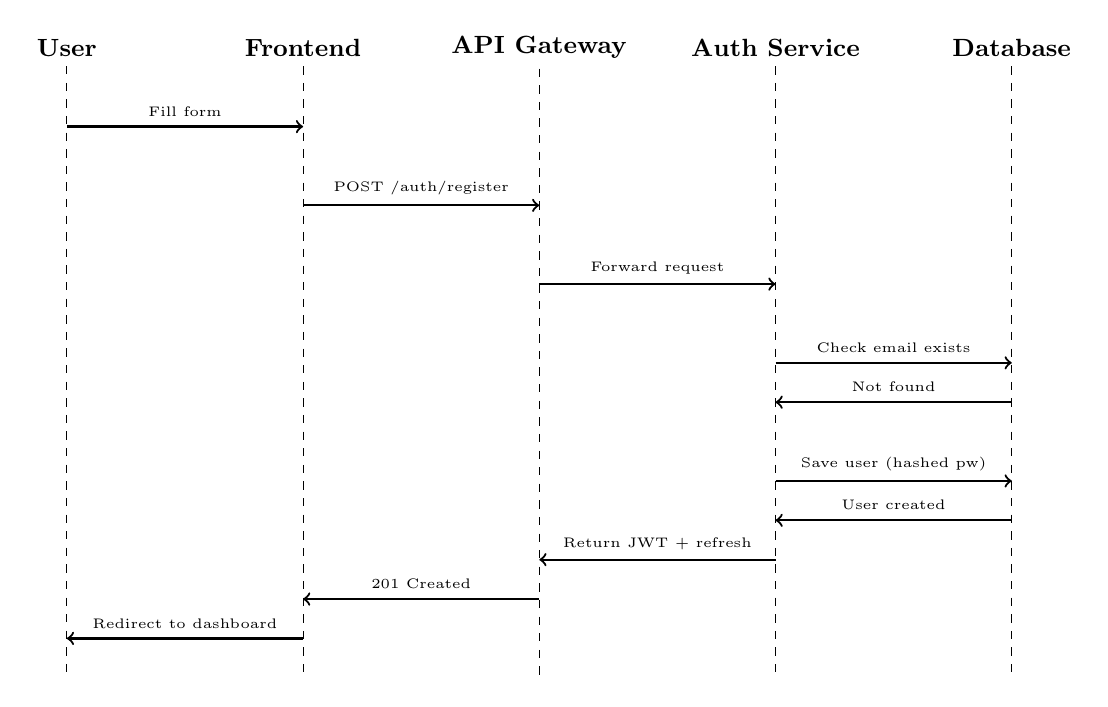
\begin{tikzpicture}[font=\small]
  % Lifelines
  \node (user) at (0, 0) {\textbf{User}};
  \node (front) at (3, 0) {\textbf{Frontend}};
  \node (gate) at (6, 0) {\textbf{API Gateway}};
  \node (auth) at (9, 0) {\textbf{Auth Service}};
  \node (db) at (12, 0) {\textbf{Database}};
  
  \draw[dashed] (user) -- (0, -8);
  \draw[dashed] (front) -- (3, -8);
  \draw[dashed] (gate) -- (6, -8);
  \draw[dashed] (auth) -- (9, -8);
  \draw[dashed] (db) -- (12, -8);
  
  % Messages
  \draw[->, thick] (0, -1) -- node[above, font=\tiny] {Fill form} (3, -1);
  \draw[->, thick] (3, -2) -- node[above, font=\tiny] {POST /auth/register} (6, -2);
  \draw[->, thick] (6, -3) -- node[above, font=\tiny] {Forward request} (9, -3);
  \draw[->, thick] (9, -4) -- node[above, font=\tiny] {Check email exists} (12, -4);
  \draw[<-, thick] (9, -4.5) -- node[above, font=\tiny] {Not found} (12, -4.5);
  \draw[->, thick] (9, -5.5) -- node[above, font=\tiny] {Save user (hashed pw)} (12, -5.5);
  \draw[<-, thick] (9, -6) -- node[above, font=\tiny] {User created} (12, -6);
  \draw[<-, thick] (6, -6.5) -- node[above, font=\tiny] {Return JWT + refresh} (9, -6.5);
  \draw[<-, thick] (3, -7) -- node[above, font=\tiny] {201 Created} (6, -7);
  \draw[<-, thick] (0, -7.5) -- node[above, font=\tiny] {Redirect to dashboard} (3, -7.5);
\end{tikzpicture}
\caption{Sequence diagram — User registration}
\label{fig:seq-register}
\end{figure}

\subsection{Sequence Diagram — Login}

\begin{figure}[H]
\centering
\begin{tikzpicture}[font=\small]
  % Lifelines
  \node (user) at (0, 0) {\textbf{User}};
  \node (front) at (3, 0) {\textbf{Frontend}};
  \node (gate) at (6, 0) {\textbf{API Gateway}};
  \node (auth) at (9, 0) {\textbf{Auth Service}};
  \node (db) at (12, 0) {\textbf{Database}};
  
  \draw[dashed] (user) -- (0, -8);
  \draw[dashed] (front) -- (3, -8);
  \draw[dashed] (gate) -- (6, -8);
  \draw[dashed] (auth) -- (9, -8);
  \draw[dashed] (db) -- (12, -8);
  
  % Messages
  \draw[->, thick] (0, -1) -- node[above, font=\tiny] {Enter credentials} (3, -1);
  \draw[->, thick] (3, -2) -- node[above, font=\tiny] {POST /auth/login} (6, -2);
  \draw[->, thick] (6, -3) -- node[above, font=\tiny] {Forward request} (9, -3);
  \draw[->, thick] (9, -4) -- node[above, font=\tiny] {Find user by email} (12, -4);
  \draw[<-, thick] (9, -4.5) -- node[above, font=\tiny] {User found} (12, -4.5);
  \draw[->, thick] (9, -5) -- node[right, font=\tiny] {Compare passwords};
  \draw[->, thick] (9, -5.5) -- node[right, font=\tiny] {Generate JWT + refresh};
  \draw[<-, thick] (6, -6) -- node[above, font=\tiny] {Return tokens} (9, -6);
  \draw[<-, thick] (3, -6.5) -- node[above, font=\tiny] {200 OK + tokens} (6, -6.5);
  \draw[<-, thick] (0, -7) -- node[above, font=\tiny] {Store token, redirect} (3, -7);
\end{tikzpicture}
\caption{Sequence diagram — User login}
\label{fig:seq-login}
\end{figure}

\subsection{Class Diagram — Auth Module}

\begin{figure}[H]
\centering
\begin{tikzpicture}[font=\small,
  class/.style={draw, rectangle, minimum width=4cm, align=left}
]
  % User class
  \node[class, fill=yellow!15] (userclass) at (0, 0) {
    \textbf{User}\\
    \hline
    - id: UUID\\
    - email: String\\
    - password: String\\
    - firstName: String\\
    - lastName: String\\
    - role: Role\\
    - createdAt: DateTime\\
    - updatedAt: DateTime\\
    \hline
    + register()\\
    + login()\\
    + resetPassword()
  };
  
  % Role enum
  \node[class, fill=green!15] (roleenum) at (6, 0) {
    \textbf{<<enum>> Role}\\
    \hline
    USER\\
    ADMIN
  };
  
  % RefreshToken class
  \node[class, fill=blue!15] (tokenclass) at (0, -5.5) {
    \textbf{RefreshToken}\\
    \hline
    - id: UUID\\
    - token: String\\
    - userId: UUID\\
    - expiresAt: DateTime\\
    - isRevoked: Boolean\\
    \hline
    + revoke()
  };
  
  % Relations
  \draw[->, thick] (userclass) -- node[above, font=\tiny] {has} (roleenum);
  \draw[->, thick] (userclass) -- node[left, font=\tiny] {has many} (tokenclass);
\end{tikzpicture}
\caption{Class diagram — Authentication module}
\label{fig:class-auth}
\end{figure}

\subsection{Implementation Screenshots}

% INSERT ACTUAL SCREENSHOTS HERE
\begin{figure}[H]
\centering
\fbox{\parbox{0.9\textwidth}{\centering\vspace{3cm}\textit{Insert registration page screenshot}\vspace{3cm}}}
\caption{Registration page}
\label{fig:register-page}
\end{figure}

\begin{figure}[H]
\centering
\fbox{\parbox{0.9\textwidth}{\centering\vspace{3cm}\textit{Insert login page screenshot}\vspace{3cm}}}
\caption{Login page}
\label{fig:login-page}
\end{figure}

\subsection{Sprint 2 Review}

At the end of Sprint 2, the following deliverables were achieved:
\begin{itemize}
  \item Complete auth service with registration, login, logout, password reset.
  \item JWT + refresh token implementation with role-based guards.
  \item Login and registration pages with form validation.
  \item OpenNebula installed and configured on the server.
  \item KVM hypervisor operational with VM templates.
\end{itemize}

% ============================================================
\section{Conclusion}

In this chapter, we completed the first two sprints. Sprint 1 established the project foundation with a modern landing page and Docker-based development environment. Sprint 2 delivered a complete authentication system with secure JWT-based access control. On the infrastructure side, OpenNebula was installed and configured for VM provisioning.

In the next chapter, we will cover Sprint 3 (User Management \& Dashboard) and Sprint 4 (VM Management \& Worker Service).

% ============================================================
\chapter{Sprint 1 \& Sprint 2: Foundation and Authentication}

\section{Introduction}

This chapter covers the first two sprints of the project. Sprint 1 focuses on establishing the project foundation and building the landing page, while Sprint 2 implements the authentication service with JWT-based security.

% ============================================================
% SPRINT 1
% ============================================================
\section{Sprint 1: Landing Page \& Project Foundation}

\sprintcard{1}{Landing Page \& Project Foundation}{Deliver a responsive landing page and set up the project skeleton with Docker containers.}

\subsection{Sprint Backlog}

\begin{longtable}{|c|p{5cm}|c|c|c|}
\hline
\rowcolor{blue!15}
\textbf{Task ID} & \textbf{Task} & \textbf{Assignee} & \textbf{Est.} & \textbf{Status} \\
\hline
\endhead
T-1.1 & Scaffold Next.js project & DSI & 2h & Done \\
\hline
T-1.2 & Scaffold NestJS microservices & DSI & 4h & Done \\
\hline
T-1.3 & Setup Docker Compose & DSI & 3h & Done \\
\hline
T-1.4 & Setup PostgreSQL + ORM & DSI & 3h & Done \\
\hline
T-1.5 & Landing page — Hero section & DSI & 4h & Done \\
\hline
T-1.6 & Landing page — Pricing section & DSI & 4h & Done \\
\hline
T-1.7 & Landing page — Features + Footer & DSI & 3h & Done \\
\hline
T-1.8 & Responsive design + Polish & DSI & 4h & Done \\
\hline
T-1.9 & Ubuntu Server hardening & RSI & 4h & Done \\
\hline
T-1.10 & Network configuration & RSI & 3h & Done \\
\hline
T-1.11 & Docker install on server & RSI & 2h & Done \\
\hline
T-1.12 & OpenNebula research & RSI & 6h & Done \\
\hline
\caption{Sprint 1 backlog}
\label{tab:sprint1-backlog}
\end{longtable}

\subsection{Mockups and Design}

% INSERT FIGMA SCREENSHOTS HERE
\begin{figure}[H]
\centering
% \includegraphics[width=\textwidth]{images/landing-mockup.png}
\fbox{\parbox{0.9\textwidth}{\centering\vspace{3cm}\textit{Insert Figma landing page mockup here}\vspace{3cm}}}
\caption{Landing page mockup (Figma)}
\label{fig:landing-mockup}
\end{figure}

\subsection{Implementation}

\subsubsection{Project Structure}

The project follows a monorepo structure with separate directories for each microservice:

\begin{lstlisting}[language=bash, caption={Project directory structure}]
cloudvm/
├── frontend/          # Next.js application
├── services/
│   ├── gateway/       # API Gateway (NestJS)
│   ├── auth/          # Auth Service (NestJS)
│   ├── user/          # User Service (NestJS)
│   ├── vm/            # VM Service (NestJS)
│   └── payment/       # Payment Service (NestJS)
├── worker/            # Python Worker
├── docker-compose.yml
└── .env
\end{lstlisting}

\subsubsection{Landing Page Screenshots}

% INSERT ACTUAL SCREENSHOTS HERE
\begin{figure}[H]
\centering
\fbox{\parbox{0.9\textwidth}{\centering\vspace{3cm}\textit{Insert landing page hero section screenshot}\vspace{3cm}}}
\caption{Landing page — Hero section}
\label{fig:landing-hero}
\end{figure}

\begin{figure}[H]
\centering
\fbox{\parbox{0.9\textwidth}{\centering\vspace{3cm}\textit{Insert landing page pricing section screenshot}\vspace{3cm}}}
\caption{Landing page — Pricing section}
\label{fig:landing-pricing}
\end{figure}

\subsection{Sprint 1 Review}

At the end of Sprint 1, the following deliverables were achieved:
\begin{itemize}
  \item Responsive landing page with hero, features, pricing, and footer sections.
  \item Docker Compose configuration with containers for all microservices.
  \item PostgreSQL database initialized with ORM configuration.
  \item Ubuntu Server hardened with SSH key authentication.
  \item Docker installed and configured on the server.
\end{itemize}


% ============================================================
% SPRINT 2
% ============================================================
\section{Sprint 2: Authentication Service}

\sprintcard{2}{Authentication Service}{Implement secure user registration, login, JWT authentication, and role-based access control.}

\subsection{Sprint Backlog}

\begin{longtable}{|c|p{5cm}|c|c|c|}
\hline
\rowcolor{blue!15}
\textbf{Task ID} & \textbf{Task} & \textbf{Assignee} & \textbf{Est.} & \textbf{Status} \\
\hline
\endhead
T-2.1 & Registration endpoint & DSI & 4h & Done \\
\hline
T-2.2 & Login endpoint & DSI & 4h & Done \\
\hline
T-2.3 & JWT + Refresh tokens & DSI & 4h & Done \\
\hline
T-2.4 & Logout + token blacklist & DSI & 2h & Done \\
\hline
T-2.5 & Password reset flow & DSI & 3h & Done \\
\hline
T-2.6 & Auth guards (JWT, Role) & DSI & 3h & Done \\
\hline
T-2.7 & Register page (frontend) & DSI & 4h & Done \\
\hline
T-2.8 & Login page (frontend) & DSI & 3h & Done \\
\hline
T-2.9 & Auth state management & DSI & 3h & Done \\
\hline
T-2.10 & OpenNebula installation & RSI & 6h & Done \\
\hline
T-2.11 & OpenNebula configuration & RSI & 6h & Done \\
\hline
T-2.12 & KVM setup + VM templates & RSI & 6h & Done \\
\hline
\caption{Sprint 2 backlog}
\label{tab:sprint2-backlog}
\end{longtable}

\subsection{Use Case Diagram — Authentication}

\begin{figure}[H]
\centering
\begin{tikzpicture}[
  usecase/.style={draw, ellipse, minimum width=3cm, minimum height=0.8cm, align=center, font=\scriptsize}
]
  % System boundary
  \draw[thick, rounded corners] (0, -5) rectangle (6, 0.5);
  \node[font=\small\bfseries] at (3, 0.2) {Authentication Module};
  
  % Actor
  \node (visitor) at (-2, -2) {Visitor};
  
  % Use cases
  \node[usecase] (uc1) at (3, -0.5) {Register};
  \node[usecase] (uc2) at (3, -1.5) {Login};
  \node[usecase] (uc3) at (3, -2.5) {Logout};
  \node[usecase] (uc4) at (3, -3.5) {Reset Password};
  \node[usecase] (uc5) at (3, -4.5) {Refresh Token};
  
  % Arrows
  \draw (visitor) -- (uc1);
  \draw (visitor) -- (uc2);
  \draw (visitor) -- (uc3);
  \draw (visitor) -- (uc4);
  \draw[dashed] (uc2) -- node[right, font=\tiny] {<<include>>} (uc5);
  
\end{tikzpicture}
\caption{Use case diagram — Authentication}
\label{fig:uc-auth}
\end{figure}

\subsection{Sequence Diagram — Registration}

\begin{figure}[H]
\centering
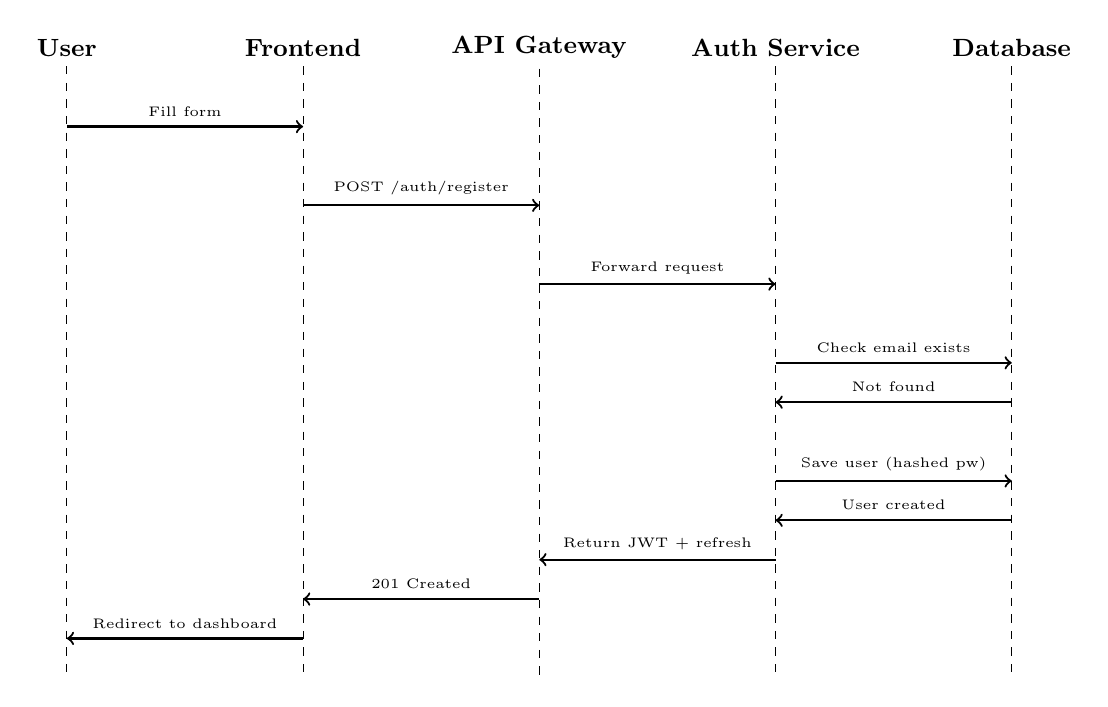
\begin{tikzpicture}[font=\small]
  % Lifelines
  \node (user) at (0, 0) {\textbf{User}};
  \node (front) at (3, 0) {\textbf{Frontend}};
  \node (gate) at (6, 0) {\textbf{API Gateway}};
  \node (auth) at (9, 0) {\textbf{Auth Service}};
  \node (db) at (12, 0) {\textbf{Database}};
  
  \draw[dashed] (user) -- (0, -8);
  \draw[dashed] (front) -- (3, -8);
  \draw[dashed] (gate) -- (6, -8);
  \draw[dashed] (auth) -- (9, -8);
  \draw[dashed] (db) -- (12, -8);
  
  % Messages
  \draw[->, thick] (0, -1) -- node[above, font=\tiny] {Fill form} (3, -1);
  \draw[->, thick] (3, -2) -- node[above, font=\tiny] {POST /auth/register} (6, -2);
  \draw[->, thick] (6, -3) -- node[above, font=\tiny] {Forward request} (9, -3);
  \draw[->, thick] (9, -4) -- node[above, font=\tiny] {Check email exists} (12, -4);
  \draw[<-, thick] (9, -4.5) -- node[above, font=\tiny] {Not found} (12, -4.5);
  \draw[->, thick] (9, -5.5) -- node[above, font=\tiny] {Save user (hashed pw)} (12, -5.5);
  \draw[<-, thick] (9, -6) -- node[above, font=\tiny] {User created} (12, -6);
  \draw[<-, thick] (6, -6.5) -- node[above, font=\tiny] {Return JWT + refresh} (9, -6.5);
  \draw[<-, thick] (3, -7) -- node[above, font=\tiny] {201 Created} (6, -7);
  \draw[<-, thick] (0, -7.5) -- node[above, font=\tiny] {Redirect to dashboard} (3, -7.5);
\end{tikzpicture}
\caption{Sequence diagram — User registration}
\label{fig:seq-register}
\end{figure}

\subsection{Sequence Diagram — Login}

\begin{figure}[H]
\centering
\begin{tikzpicture}[font=\small]
  % Lifelines
  \node (user) at (0, 0) {\textbf{User}};
  \node (front) at (3, 0) {\textbf{Frontend}};
  \node (gate) at (6, 0) {\textbf{API Gateway}};
  \node (auth) at (9, 0) {\textbf{Auth Service}};
  \node (db) at (12, 0) {\textbf{Database}};
  
  \draw[dashed] (user) -- (0, -8);
  \draw[dashed] (front) -- (3, -8);
  \draw[dashed] (gate) -- (6, -8);
  \draw[dashed] (auth) -- (9, -8);
  \draw[dashed] (db) -- (12, -8);
  
  % Messages
  \draw[->, thick] (0, -1) -- node[above, font=\tiny] {Enter credentials} (3, -1);
  \draw[->, thick] (3, -2) -- node[above, font=\tiny] {POST /auth/login} (6, -2);
  \draw[->, thick] (6, -3) -- node[above, font=\tiny] {Forward request} (9, -3);
  \draw[->, thick] (9, -4) -- node[above, font=\tiny] {Find user by email} (12, -4);
  \draw[<-, thick] (9, -4.5) -- node[above, font=\tiny] {User found} (12, -4.5);
  \draw[->, thick] (9, -5) -- node[right, font=\tiny] {Compare passwords};
  \draw[->, thick] (9, -5.5) -- node[right, font=\tiny] {Generate JWT + refresh};
  \draw[<-, thick] (6, -6) -- node[above, font=\tiny] {Return tokens} (9, -6);
  \draw[<-, thick] (3, -6.5) -- node[above, font=\tiny] {200 OK + tokens} (6, -6.5);
  \draw[<-, thick] (0, -7) -- node[above, font=\tiny] {Store token, redirect} (3, -7);
\end{tikzpicture}
\caption{Sequence diagram — User login}
\label{fig:seq-login}
\end{figure}

\subsection{Class Diagram — Auth Module}

\begin{figure}[H]
\centering
\begin{tikzpicture}[font=\small,
  class/.style={draw, rectangle, minimum width=4cm, align=left}
]
  % User class
  \node[class, fill=yellow!15] (userclass) at (0, 0) {
    \textbf{User}\\
    \hline
    - id: UUID\\
    - email: String\\
    - password: String\\
    - firstName: String\\
    - lastName: String\\
    - role: Role\\
    - createdAt: DateTime\\
    - updatedAt: DateTime\\
    \hline
    + register()\\
    + login()\\
    + resetPassword()
  };
  
  % Role enum
  \node[class, fill=green!15] (roleenum) at (6, 0) {
    \textbf{<<enum>> Role}\\
    \hline
    USER\\
    ADMIN
  };
  
  % RefreshToken class
  \node[class, fill=blue!15] (tokenclass) at (0, -5.5) {
    \textbf{RefreshToken}\\
    \hline
    - id: UUID\\
    - token: String\\
    - userId: UUID\\
    - expiresAt: DateTime\\
    - isRevoked: Boolean\\
    \hline
    + revoke()
  };
  
  % Relations
  \draw[->, thick] (userclass) -- node[above, font=\tiny] {has} (roleenum);
  \draw[->, thick] (userclass) -- node[left, font=\tiny] {has many} (tokenclass);
\end{tikzpicture}
\caption{Class diagram — Authentication module}
\label{fig:class-auth}
\end{figure}

\subsection{Implementation Screenshots}

% INSERT ACTUAL SCREENSHOTS HERE
\begin{figure}[H]
\centering
\fbox{\parbox{0.9\textwidth}{\centering\vspace{3cm}\textit{Insert registration page screenshot}\vspace{3cm}}}
\caption{Registration page}
\label{fig:register-page}
\end{figure}

\begin{figure}[H]
\centering
\fbox{\parbox{0.9\textwidth}{\centering\vspace{3cm}\textit{Insert login page screenshot}\vspace{3cm}}}
\caption{Login page}
\label{fig:login-page}
\end{figure}

\subsection{Sprint 2 Review}

At the end of Sprint 2, the following deliverables were achieved:
\begin{itemize}
  \item Complete auth service with registration, login, logout, password reset.
  \item JWT + refresh token implementation with role-based guards.
  \item Login and registration pages with form validation.
  \item OpenNebula installed and configured on the server.
  \item KVM hypervisor operational with VM templates.
\end{itemize}

% ============================================================
\section{Conclusion}

In this chapter, we completed the first two sprints. Sprint 1 established the project foundation with a modern landing page and Docker-based development environment. Sprint 2 delivered a complete authentication system with secure JWT-based access control. On the infrastructure side, OpenNebula was installed and configured for VM provisioning.

In the next chapter, we will cover Sprint 3 (User Management \& Dashboard) and Sprint 4 (VM Management \& Worker Service).

% ============================================================
\chapter{Sprint 1 \& Sprint 2: Foundation and Authentication}

\section{Introduction}

This chapter covers the first two sprints of the project. Sprint 1 focuses on establishing the project foundation and building the landing page, while Sprint 2 implements the authentication service with JWT-based security.

% ============================================================
% SPRINT 1
% ============================================================
\section{Sprint 1: Landing Page \& Project Foundation}

\sprintcard{1}{Landing Page \& Project Foundation}{Deliver a responsive landing page and set up the project skeleton with Docker containers.}

\subsection{Sprint Backlog}

\begin{longtable}{|c|p{5cm}|c|c|c|}
\hline
\rowcolor{blue!15}
\textbf{Task ID} & \textbf{Task} & \textbf{Assignee} & \textbf{Est.} & \textbf{Status} \\
\hline
\endhead
T-1.1 & Scaffold Next.js project & DSI & 2h & Done \\
\hline
T-1.2 & Scaffold NestJS microservices & DSI & 4h & Done \\
\hline
T-1.3 & Setup Docker Compose & DSI & 3h & Done \\
\hline
T-1.4 & Setup PostgreSQL + ORM & DSI & 3h & Done \\
\hline
T-1.5 & Landing page — Hero section & DSI & 4h & Done \\
\hline
T-1.6 & Landing page — Pricing section & DSI & 4h & Done \\
\hline
T-1.7 & Landing page — Features + Footer & DSI & 3h & Done \\
\hline
T-1.8 & Responsive design + Polish & DSI & 4h & Done \\
\hline
T-1.9 & Ubuntu Server hardening & RSI & 4h & Done \\
\hline
T-1.10 & Network configuration & RSI & 3h & Done \\
\hline
T-1.11 & Docker install on server & RSI & 2h & Done \\
\hline
T-1.12 & OpenNebula research & RSI & 6h & Done \\
\hline
\caption{Sprint 1 backlog}
\label{tab:sprint1-backlog}
\end{longtable}

\subsection{Mockups and Design}

% INSERT FIGMA SCREENSHOTS HERE
\begin{figure}[H]
\centering
% \includegraphics[width=\textwidth]{images/landing-mockup.png}
\fbox{\parbox{0.9\textwidth}{\centering\vspace{3cm}\textit{Insert Figma landing page mockup here}\vspace{3cm}}}
\caption{Landing page mockup (Figma)}
\label{fig:landing-mockup}
\end{figure}

\subsection{Implementation}

\subsubsection{Project Structure}

The project follows a monorepo structure with separate directories for each microservice:

\begin{lstlisting}[language=bash, caption={Project directory structure}]
cloudvm/
├── frontend/          # Next.js application
├── services/
│   ├── gateway/       # API Gateway (NestJS)
│   ├── auth/          # Auth Service (NestJS)
│   ├── user/          # User Service (NestJS)
│   ├── vm/            # VM Service (NestJS)
│   └── payment/       # Payment Service (NestJS)
├── worker/            # Python Worker
├── docker-compose.yml
└── .env
\end{lstlisting}

\subsubsection{Landing Page Screenshots}

% INSERT ACTUAL SCREENSHOTS HERE
\begin{figure}[H]
\centering
\fbox{\parbox{0.9\textwidth}{\centering\vspace{3cm}\textit{Insert landing page hero section screenshot}\vspace{3cm}}}
\caption{Landing page — Hero section}
\label{fig:landing-hero}
\end{figure}

\begin{figure}[H]
\centering
\fbox{\parbox{0.9\textwidth}{\centering\vspace{3cm}\textit{Insert landing page pricing section screenshot}\vspace{3cm}}}
\caption{Landing page — Pricing section}
\label{fig:landing-pricing}
\end{figure}

\subsection{Sprint 1 Review}

At the end of Sprint 1, the following deliverables were achieved:
\begin{itemize}
  \item Responsive landing page with hero, features, pricing, and footer sections.
  \item Docker Compose configuration with containers for all microservices.
  \item PostgreSQL database initialized with ORM configuration.
  \item Ubuntu Server hardened with SSH key authentication.
  \item Docker installed and configured on the server.
\end{itemize}


% ============================================================
% SPRINT 2
% ============================================================
\section{Sprint 2: Authentication Service}

\sprintcard{2}{Authentication Service}{Implement secure user registration, login, JWT authentication, and role-based access control.}

\subsection{Sprint Backlog}

\begin{longtable}{|c|p{5cm}|c|c|c|}
\hline
\rowcolor{blue!15}
\textbf{Task ID} & \textbf{Task} & \textbf{Assignee} & \textbf{Est.} & \textbf{Status} \\
\hline
\endhead
T-2.1 & Registration endpoint & DSI & 4h & Done \\
\hline
T-2.2 & Login endpoint & DSI & 4h & Done \\
\hline
T-2.3 & JWT + Refresh tokens & DSI & 4h & Done \\
\hline
T-2.4 & Logout + token blacklist & DSI & 2h & Done \\
\hline
T-2.5 & Password reset flow & DSI & 3h & Done \\
\hline
T-2.6 & Auth guards (JWT, Role) & DSI & 3h & Done \\
\hline
T-2.7 & Register page (frontend) & DSI & 4h & Done \\
\hline
T-2.8 & Login page (frontend) & DSI & 3h & Done \\
\hline
T-2.9 & Auth state management & DSI & 3h & Done \\
\hline
T-2.10 & OpenNebula installation & RSI & 6h & Done \\
\hline
T-2.11 & OpenNebula configuration & RSI & 6h & Done \\
\hline
T-2.12 & KVM setup + VM templates & RSI & 6h & Done \\
\hline
\caption{Sprint 2 backlog}
\label{tab:sprint2-backlog}
\end{longtable}

\subsection{Use Case Diagram — Authentication}

\begin{figure}[H]
\centering
\begin{tikzpicture}[
  usecase/.style={draw, ellipse, minimum width=3cm, minimum height=0.8cm, align=center, font=\scriptsize}
]
  % System boundary
  \draw[thick, rounded corners] (0, -5) rectangle (6, 0.5);
  \node[font=\small\bfseries] at (3, 0.2) {Authentication Module};
  
  % Actor
  \node (visitor) at (-2, -2) {Visitor};
  
  % Use cases
  \node[usecase] (uc1) at (3, -0.5) {Register};
  \node[usecase] (uc2) at (3, -1.5) {Login};
  \node[usecase] (uc3) at (3, -2.5) {Logout};
  \node[usecase] (uc4) at (3, -3.5) {Reset Password};
  \node[usecase] (uc5) at (3, -4.5) {Refresh Token};
  
  % Arrows
  \draw (visitor) -- (uc1);
  \draw (visitor) -- (uc2);
  \draw (visitor) -- (uc3);
  \draw (visitor) -- (uc4);
  \draw[dashed] (uc2) -- node[right, font=\tiny] {<<include>>} (uc5);
  
\end{tikzpicture}
\caption{Use case diagram — Authentication}
\label{fig:uc-auth}
\end{figure}

\subsection{Sequence Diagram — Registration}

\begin{figure}[H]
\centering
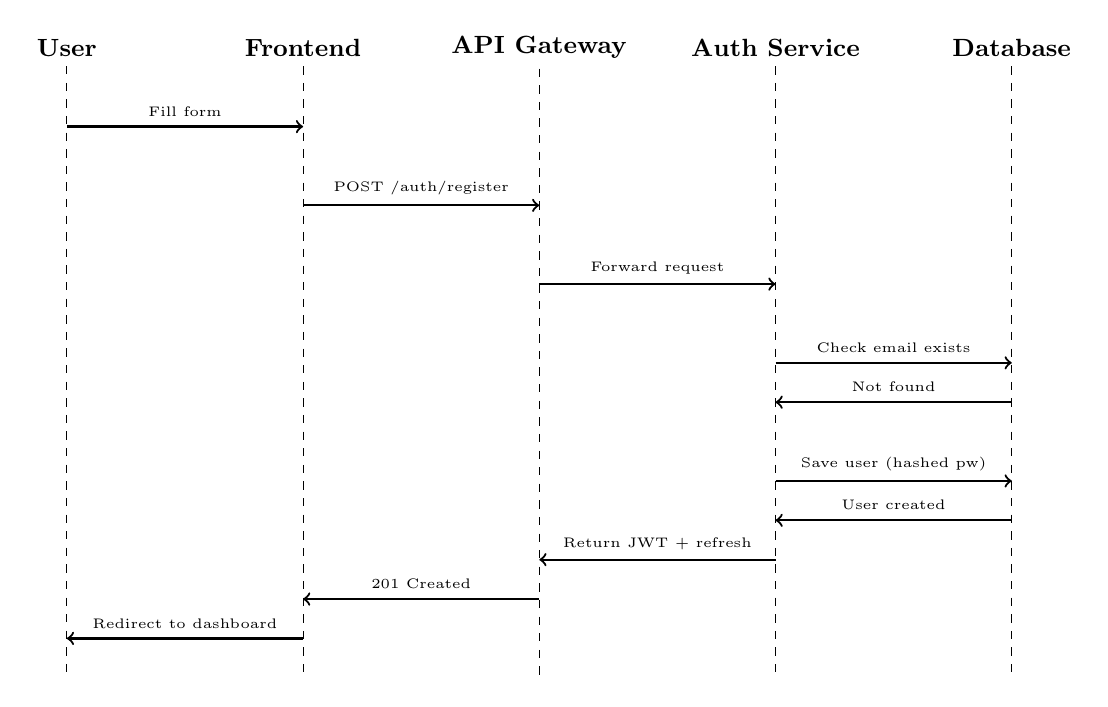
\begin{tikzpicture}[font=\small]
  % Lifelines
  \node (user) at (0, 0) {\textbf{User}};
  \node (front) at (3, 0) {\textbf{Frontend}};
  \node (gate) at (6, 0) {\textbf{API Gateway}};
  \node (auth) at (9, 0) {\textbf{Auth Service}};
  \node (db) at (12, 0) {\textbf{Database}};
  
  \draw[dashed] (user) -- (0, -8);
  \draw[dashed] (front) -- (3, -8);
  \draw[dashed] (gate) -- (6, -8);
  \draw[dashed] (auth) -- (9, -8);
  \draw[dashed] (db) -- (12, -8);
  
  % Messages
  \draw[->, thick] (0, -1) -- node[above, font=\tiny] {Fill form} (3, -1);
  \draw[->, thick] (3, -2) -- node[above, font=\tiny] {POST /auth/register} (6, -2);
  \draw[->, thick] (6, -3) -- node[above, font=\tiny] {Forward request} (9, -3);
  \draw[->, thick] (9, -4) -- node[above, font=\tiny] {Check email exists} (12, -4);
  \draw[<-, thick] (9, -4.5) -- node[above, font=\tiny] {Not found} (12, -4.5);
  \draw[->, thick] (9, -5.5) -- node[above, font=\tiny] {Save user (hashed pw)} (12, -5.5);
  \draw[<-, thick] (9, -6) -- node[above, font=\tiny] {User created} (12, -6);
  \draw[<-, thick] (6, -6.5) -- node[above, font=\tiny] {Return JWT + refresh} (9, -6.5);
  \draw[<-, thick] (3, -7) -- node[above, font=\tiny] {201 Created} (6, -7);
  \draw[<-, thick] (0, -7.5) -- node[above, font=\tiny] {Redirect to dashboard} (3, -7.5);
\end{tikzpicture}
\caption{Sequence diagram — User registration}
\label{fig:seq-register}
\end{figure}

\subsection{Sequence Diagram — Login}

\begin{figure}[H]
\centering
\begin{tikzpicture}[font=\small]
  % Lifelines
  \node (user) at (0, 0) {\textbf{User}};
  \node (front) at (3, 0) {\textbf{Frontend}};
  \node (gate) at (6, 0) {\textbf{API Gateway}};
  \node (auth) at (9, 0) {\textbf{Auth Service}};
  \node (db) at (12, 0) {\textbf{Database}};
  
  \draw[dashed] (user) -- (0, -8);
  \draw[dashed] (front) -- (3, -8);
  \draw[dashed] (gate) -- (6, -8);
  \draw[dashed] (auth) -- (9, -8);
  \draw[dashed] (db) -- (12, -8);
  
  % Messages
  \draw[->, thick] (0, -1) -- node[above, font=\tiny] {Enter credentials} (3, -1);
  \draw[->, thick] (3, -2) -- node[above, font=\tiny] {POST /auth/login} (6, -2);
  \draw[->, thick] (6, -3) -- node[above, font=\tiny] {Forward request} (9, -3);
  \draw[->, thick] (9, -4) -- node[above, font=\tiny] {Find user by email} (12, -4);
  \draw[<-, thick] (9, -4.5) -- node[above, font=\tiny] {User found} (12, -4.5);
  \draw[->, thick] (9, -5) -- node[right, font=\tiny] {Compare passwords};
  \draw[->, thick] (9, -5.5) -- node[right, font=\tiny] {Generate JWT + refresh};
  \draw[<-, thick] (6, -6) -- node[above, font=\tiny] {Return tokens} (9, -6);
  \draw[<-, thick] (3, -6.5) -- node[above, font=\tiny] {200 OK + tokens} (6, -6.5);
  \draw[<-, thick] (0, -7) -- node[above, font=\tiny] {Store token, redirect} (3, -7);
\end{tikzpicture}
\caption{Sequence diagram — User login}
\label{fig:seq-login}
\end{figure}

\subsection{Class Diagram — Auth Module}

\begin{figure}[H]
\centering
\begin{tikzpicture}[font=\small,
  class/.style={draw, rectangle, minimum width=4cm, align=left}
]
  % User class
  \node[class, fill=yellow!15] (userclass) at (0, 0) {
    \textbf{User}\\
    \hline
    - id: UUID\\
    - email: String\\
    - password: String\\
    - firstName: String\\
    - lastName: String\\
    - role: Role\\
    - createdAt: DateTime\\
    - updatedAt: DateTime\\
    \hline
    + register()\\
    + login()\\
    + resetPassword()
  };
  
  % Role enum
  \node[class, fill=green!15] (roleenum) at (6, 0) {
    \textbf{<<enum>> Role}\\
    \hline
    USER\\
    ADMIN
  };
  
  % RefreshToken class
  \node[class, fill=blue!15] (tokenclass) at (0, -5.5) {
    \textbf{RefreshToken}\\
    \hline
    - id: UUID\\
    - token: String\\
    - userId: UUID\\
    - expiresAt: DateTime\\
    - isRevoked: Boolean\\
    \hline
    + revoke()
  };
  
  % Relations
  \draw[->, thick] (userclass) -- node[above, font=\tiny] {has} (roleenum);
  \draw[->, thick] (userclass) -- node[left, font=\tiny] {has many} (tokenclass);
\end{tikzpicture}
\caption{Class diagram — Authentication module}
\label{fig:class-auth}
\end{figure}

\subsection{Implementation Screenshots}

% INSERT ACTUAL SCREENSHOTS HERE
\begin{figure}[H]
\centering
\fbox{\parbox{0.9\textwidth}{\centering\vspace{3cm}\textit{Insert registration page screenshot}\vspace{3cm}}}
\caption{Registration page}
\label{fig:register-page}
\end{figure}

\begin{figure}[H]
\centering
\fbox{\parbox{0.9\textwidth}{\centering\vspace{3cm}\textit{Insert login page screenshot}\vspace{3cm}}}
\caption{Login page}
\label{fig:login-page}
\end{figure}

\subsection{Sprint 2 Review}

At the end of Sprint 2, the following deliverables were achieved:
\begin{itemize}
  \item Complete auth service with registration, login, logout, password reset.
  \item JWT + refresh token implementation with role-based guards.
  \item Login and registration pages with form validation.
  \item OpenNebula installed and configured on the server.
  \item KVM hypervisor operational with VM templates.
\end{itemize}

% ============================================================
\section{Conclusion}

In this chapter, we completed the first two sprints. Sprint 1 established the project foundation with a modern landing page and Docker-based development environment. Sprint 2 delivered a complete authentication system with secure JWT-based access control. On the infrastructure side, OpenNebula was installed and configured for VM provisioning.

In the next chapter, we will cover Sprint 3 (User Management \& Dashboard) and Sprint 4 (VM Management \& Worker Service).
